% "{'classe':('PSI'),'chapitre':'cin_geo','type':('td','todo'),'titre':'Exosquelette Atalante', 'source':'CCS PSI 2023','comp':('GEO-03'),'corrige':True}"
\setchapterimage{fig_00.jpg}
\chapter*{TD \arabic{cptTD} \\ 
Exosquelette Atalante -- \ifprof Corrigé \else Sujet \fi}
\addcontentsline{toc}{section}{TD \arabic{cptTD} : 
Exosquelette Atalante -- \ifprof Corrigé \else Sujet \fi}

\iflivret \stepcounter{cptTD} \else
\ifprof  \stepcounter{cptTD} \else \fi
\fi



\marginnote{\textit{D'après CCS PSI 2023.}}
\marginnote{\xpComp{GEO}{03}}


\ifprof
\else
\begin{marginfigure}
\centering
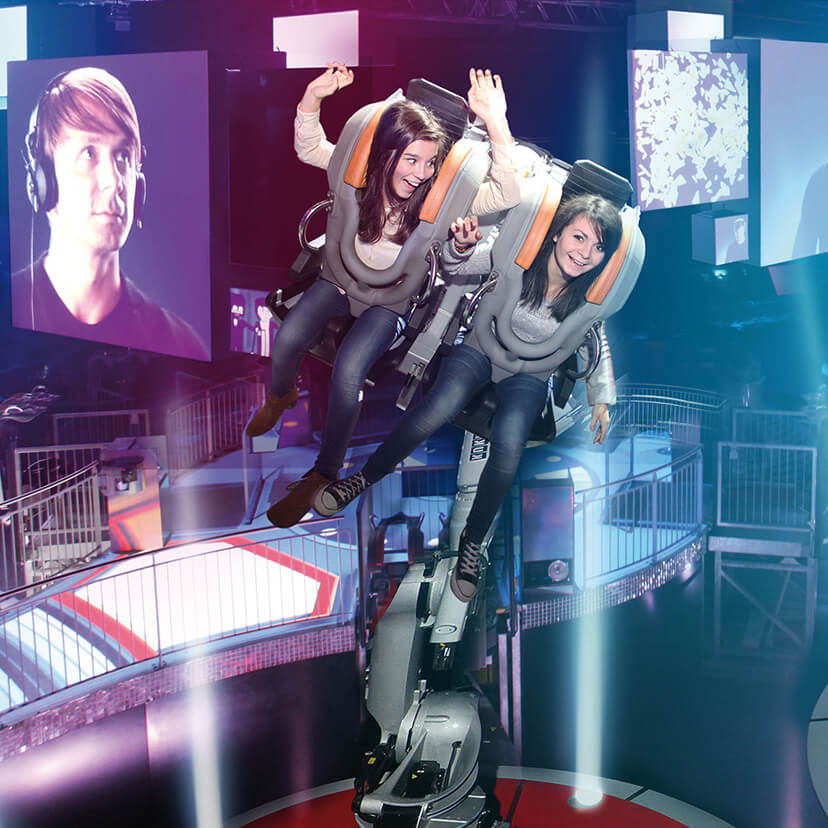
\includegraphics[width=.5\linewidth]{fig_01}
\end{marginfigure}

%En phase de rééducation à la proprioception de la verticalité et de la marche, il est nécessaire d'éviter la chute du patient. 

Des essais, menés sur des humains valides, ont permis de mettre en avant que lors d'une marche en ligne droite, une erreur de positionnement du talon de $\pm \SI{5}{mm}$ risque d'amener à un déséquilibre, et donc à une chute (exigence 1.2.1.1, figure \ref{ccs_psi_2023_fig_02}). Il est donc nécessaire de déterminer l'erreur de positionnement angulaire admissible sur chacun des axes de l'exosquelette pour éviter cette chute.

\begin{figure}[!h]
\centering
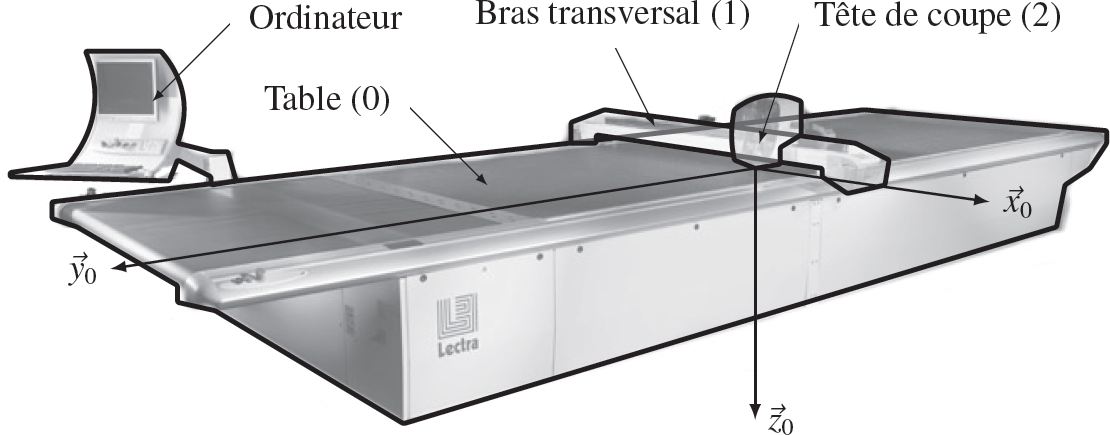
\includegraphics[width=.9\linewidth]{fig_02}
\caption{Diagramme des exigences partiel \label{ccs_psi_2023_fig_02}}
\end{figure}


Dans toute l'étude, les hypothèses et notations seront les suivantes (figure \ref{ccs_psi_2023_fig_04}) :

\begin{itemize}
  \item l'étude est menée dans le plan sagittal $\left(A, \vec{y}_{1}, \vec{z}_{1}\right)$, où $\vec{z}_{1}$ est vertical ascendant ;
  \item les différentes caractéristiques de dimension, masse et inertie des différents solides sont précisées annexe B ;
  \item le buste 1 étant animé d'un mouvement de translation rectiligne uniforme par rapport au référentiel terrestre, il est considéré comme galiléen ;
  \item l'étude se limite à la partie de la marche pour laquelle une des deux jambes est totalement décollée du sol; % (de $70 \%$ à $100 \%$ de la foulée sur la figure 3) ;
  \item le buste 1 est en liaison pivot d'axe $\left(A, \vec{x}_{1}\right)$ avec la cuisse 2 ; on note $\theta_{1}=\left(\vec{y}_{1}, \vec{y}_{2}\right)=\left(\vec{z}_{1}, \vec{z}_{2}\right)$;
  \item l'ensemble \{pied+tibia 3\} , considéré comme solidaire, est en liaison pivot d'axe $\left(B, \vec{x}_{1}\right)$ avec la cuisse 2 ; on note $\theta_{2}=\left(\vec{y}_{2}, \vec{y}_{3}\right)=\left(\vec{z}_{2}, \vec{z}_{3}\right)$;
  \item les liaisons décrites précédemment sont supposées parfaites.
\end{itemize}

\marginnote{
\begin{itemize}
\item $\vect{BA}=L_2\vz{2}$.
\item $\vect{DB}=L_3\vz{3}$.
\end{itemize}}

\begin{figure}[!h]
\centering
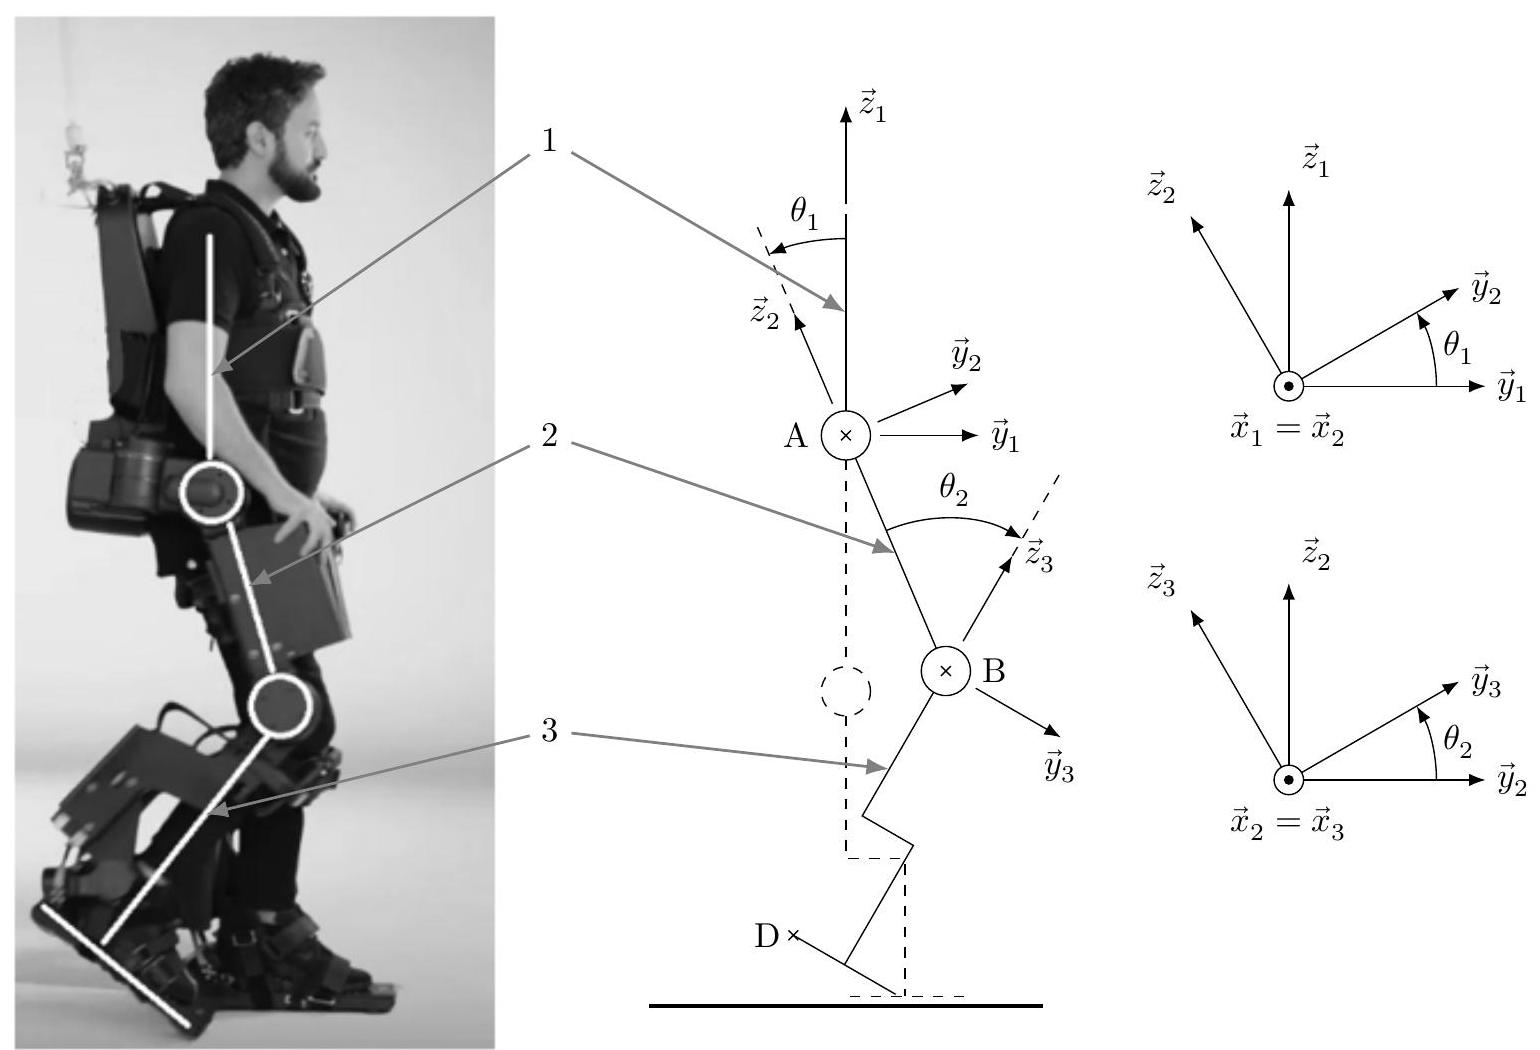
\includegraphics[width=.8\textwidth]{2023_05_12_54c6a64d2ffce28d5c72g-03}
\caption{Modélisation utilisée pour la marche en ligne droite \label{ccs_psi_2023_fig_04}}
\end{figure}
\fi

%Les positions des différents axes sont asservies à une consigne de référence afin d'obtenir la position désirée pour le point $D$ caractérisant la pointe du talon. 
\begin{obj}
Le cahier des charges impose que la position dans l'espace du point $D$ par rapport au point $A$ doive être celle désirée, avec une incertitude maximale de $S_{D}=5 \mathrm{~mm}$. 
\end{obj}
\ifprof
\else
On pose :
$$
\overrightarrow{A D}=Y \vec{y}_{1}+Z \vec{z}_{1}
$$
\fi
% Q1
\question{\label{ccs_psi_2023_q_01}Déterminer les expressions de $Y$ et $Z$, en fonction de $\theta_{1}, \theta_{2}, L_{2}$ et $L_{3}$.}
\ifprof
\begin{corrige}

\'Ecrivons la fermeture géométrique dans le triangle $ABD$ : $\vect{AD}+ \vect{DB}+\vect{BA} = \vect{0}$ soit $Y\vect{y_1}+Z\vect{z_1}+ L_3 \vect{z_3}+ L_2 \vect{z_2} = \vect{0}$.

On souhaite les expressions de $Y$ et $Z$ projetons l'expression dans la base $\left(\vect{y_1},\vect{z_1}\right)$ :

$Y\vect{y_1}+Z\vect{z_1}
+L_3 \left( \cos \left(\theta_1 + \theta_2 \right) \vect{z_1} - \sin \left(\theta_1 + \theta_2 \right) \vect{y_1}\right) 
+ L_2 \left( \cos \left(\theta_1 \right) \vect{z_1} - \sin \left(\theta_1  \right) \vect{y_1}\right)  = \vect{0}$.

On alors :
$$
\left\{
\begin{array}{l}
Y =  L_3 \sin  \left(\theta_1 + \theta_2 \right)  + L_2 \sin \left(\theta_1  \right) \\
Z =- L_3 \cos \left(\theta_1 + \theta_2 \right) - L_2 \cos \left(\theta_1 \right)  
\end{array}.
\right.
$$
\end{corrige}
\else
\fi

\ifprof
\else
L'erreur de positionnement du talon est modélisée par une variation autour d'une position connue. Cette position est paramétrée par les coordonnées $Y_{0}$ et $Z_{0}$ pour le point $D$, et par des angles $\theta_{1,0}$ et $\theta_{2,0}$ pour les liaisons pivots. Ce paramétrage se traduit, pour une variation angulaire $\Delta_{\theta}$, considérée égale sur chacun des axes, à des variations de position, $\Delta_{Y}$ et $\Delta_{Z}$, du point $D$. On suppose $\Delta_{\theta}$ faible, proche de 0 .
\fi
%Q2
\question{\label{ccs_psi_2023_q_02}  À l'aide du résultat de la question \ref{ccs_psi_2023_q_01}, écrit à la position $\left(Y_{0}, Z_{0}\right)$, puis à la position $\left(Y_{0}+\Delta_{Y}, Z_{0}+\Delta_{Z}\right)$, déterminer les expressions de $\Delta_{Y}$ et $\Delta_{Z}$, en fonction de $\theta_{1,0}, \theta_{2,0}, \Delta_{\theta}, L_{2}$ et $L_{3}$.}
\ifprof
\begin{corrige}

D'une part : 
$
\left\{
\begin{array}{l}
Y_0 =  L_3 \sin  \left(\theta_{1,0}+ \theta_{2,0} \right)  + L_2 \sin \left(\theta_{1,0}  \right) \\
Z_0 =- L_3 \cos \left(\theta_{1,0} + \theta_{2,0} \right) - L_2 \cos \left(\theta_{1,0} \right)  
\end{array}.
\right.
$


\begin{enumerate}
\item \textbf{Méthode 1 : }

D'autre part : 
$
\left\{
\begin{array}{l}
Y_0 +\Delta_{Y}=  L_3 \sin  \left(\theta_{1,0}+ \theta_{2,0} + 2\Delta_{\theta} \right)  + L_2 \sin \left(\theta_{1,0} + \Delta_{\theta} \right) \\
Z_0 +\Delta_{Z}=- L_3 \cos \left(\theta_{1,0} + \theta_{2,0}+ 2\Delta_{\theta} \right) - L_2 \cos \left(\theta_{1,0}+\Delta_{\theta} \right)  
\end{array}.
\right.
$

En faisant la différence :

$
\left\{
\begin{array}{ll}
\Delta_{Y}& =  L_3 \sin  \left(\theta_{1,0}+ \theta_{2,0} + 2\Delta_{\theta} \right)  + L_2 \sin \left(\theta_{1,0} + \Delta_{\theta} \right)  \\ 
& - L_3 \sin  \left(\theta_{1,0}+ \theta_{2,0} \right)  - L_2 \sin \left(\theta_{1,0}  \right)\\
\Delta_{Z} & =- L_3 \cos \left(\theta_{1,0} + \theta_{2,0}+ 2\Delta_{\theta} \right) - L_2 \cos \left(\theta_{1,0}+\Delta_{\theta} \right)   
\\& +  L_3 \cos \left(\theta_{1,0} + \theta_{2,0} \right) + L_2 \cos \left(\theta_{1,0} \right)
\end{array}.
\right.
$

Par suite : 

$
\left\{
\begin{array}{ll}
\Delta_{Y}=&   L_3 \left( \sin \left(\theta_{1,0}+ \theta_{2,0} \right) \cos \left( 2\Delta_{\theta} \right) + \cos \left(\theta_{1,0}+ \theta_{2,0}\right) \sin \left(2\Delta_{\theta} \right)\right) \\
                 & + L_2 \left( \sin \left(\theta_{1,0} \right) \cos \left( \Delta_{\theta} \right) + \cos \left(\theta_{1,0}\right) \sin \left(\Delta_{\theta} \right)\right) \\
& - L_3 \sin  \left(\theta_{1,0}+ \theta_{2,0} \right)  - L_2 \sin \left(\theta_{1,0}  \right)\\
\Delta_{Z}=
&- L_3 \left(\cos \left(\theta_{1,0} + \theta_{2,0}\right) \cos\left(2\Delta_{\theta} \right)
- \sin \left(\theta_{1,0} + \theta_{2,0}\right) \sin\left(2\Delta_{\theta} \right) \right) \\
&- L_2 \left(\cos \left(\theta_{1,0} \right) \cos\left(\Delta_{\theta} \right)
- \sin \left(\theta_{1,0} \right) \sin\left(\Delta_{\theta} \right) \right)\\
&  +  L_3 \cos \left(\theta_{1,0} + \theta_{2,0} \right) + L_2 \cos \left(\theta_{1,0} \right)
\end{array}.
\right.
$

et

$
\left\{
\begin{array}{ll}
\Delta_{Y}=&   L_3\cos \left(\theta_{1,0}+ \theta_{2,0}\right) \sin \left(2\Delta_{\theta} \right)
+ L_2 \cos \left(\theta_{1,0}\right) \sin \left(\Delta_{\theta} \right)\\
\Delta_{Z}=& L_3  \sin \left(\theta_{1,0} + \theta_{2,0}\right) \sin\left(2\Delta_{\theta} \right) 
+L_2 \sin \left(\theta_{1,0} \right) \sin\left(\Delta_{\theta} \right)\\
\end{array}.
\right.
$

Par suite, 
$
\left\{
\begin{array}{ll}
\Delta_{Y}=&  2\Delta_{\theta}  L_3\cos \left(\theta_{1,0}+ \theta_{2,0}\right) 
+\Delta_{\theta}  L_2 \cos \left(\theta_{1,0}\right) \\
\Delta_{Z}=& 2\Delta_{\theta} L_3  \sin \left(\theta_{1,0} + \theta_{2,0}\right)  
+L_2 \Delta_{\theta}\sin \left(\theta_{1,0} \right) \\
\end{array}.
\right.
$

\item \textbf{Méthode 2 : }

On peut également utiliser le calcul différentiel : 

$$
\left\{
\begin{array}{l}
\Delta Y=d Y=\dfrac{\partial Y}{\partial \theta_1}\vert_{\theta_{1,0},\theta_{2,0}}d\theta_1+\dfrac{\partial Y}{\partial \theta_2}\vert_{\theta_{1,0},\theta_{2,0}}\text{d}\theta_2\\
\Delta Z=d Z=\dfrac{\partial Z}{\partial \theta_1}\vert_{\theta_{1,0},\theta_{2,0}}d\theta_1+\dfrac{\partial Z}{\partial \theta_2}\vert_{\theta_{1,0},\theta_{2,0}}\text{d}\theta_2
\end{array}
\right.
$$

Avec $\text{d}\theta_1=\text{d}\theta_2=\Delta_{\theta}$

On obtient donc : 

$$
\left\{
\begin{array}{l}
\Delta Y=\Delta_{\theta}\left[L_2\cos\theta_{10}+2L_3\cos(\theta_{20}+\theta_{10})\right]\\
\Delta Z=\Delta_{\theta}\left[L_2\sin\theta_{10}+2L_3\sin(\theta_{20}+\theta_{10})\right]
\end{array}
\right.
$$

\end{enumerate}

\end{corrige}
\else
\fi

%Q3
\question{\label{ccs_psi_2023_q_03}  Déterminer alors $\Delta_{Y Z}$, la norme de la variation de positionnement total du point $D$ dans le plan $\left(\vec{y}_{1}, \vec{z}_{1}\right)$, en fonction de $\theta_{2,0}, \Delta_{\theta}, L_{2}$ et $L_{3}$.}
\ifprof
\begin{corrige}
On a : 
$\Delta_{Y}^2 + \Delta_{X}^2 = 4\Delta_{\theta}^2L_3^2 + \Delta_{\theta}^2L_2^2 
+ 4\Delta_{\theta}^2 L_2 L_3 \left( \cos \left(\theta_{1,0}+ \theta_{2,0}\right)  \cos \left(\theta_{1,0}\right)
+  \sin \left(\theta_{1,0}+ \theta_{2,0}\right)  \sin \left(\theta_{1,0}\right) \right)$

soit 
$\Delta_{YZ}^2 = \Delta_{\theta}^2 \left(4L_3^2 + L_2^2 
+ 4 L_2 L_3 \cos \left(\theta_{2,0} \right)\right)$
\end{corrige}
\else
\fi

\ifprof
\else
Le résultat de la question précédente permet alors de relier l'erreur de position du talon $S_{D}$ à l'erreur de position sur les axes $S_{\theta}$, en considérant $\Delta_{Y Z}=S_{D}$ et $\Delta_{\theta}=S_{\theta}$. La figure \ref{ccs_psi_2023_fig_05} donne les évolutions sur un pas de marche de $S_{D}$ pour plusieurs valeurs de $S_{\theta}$.

\begin{figure}[!h]
\centering
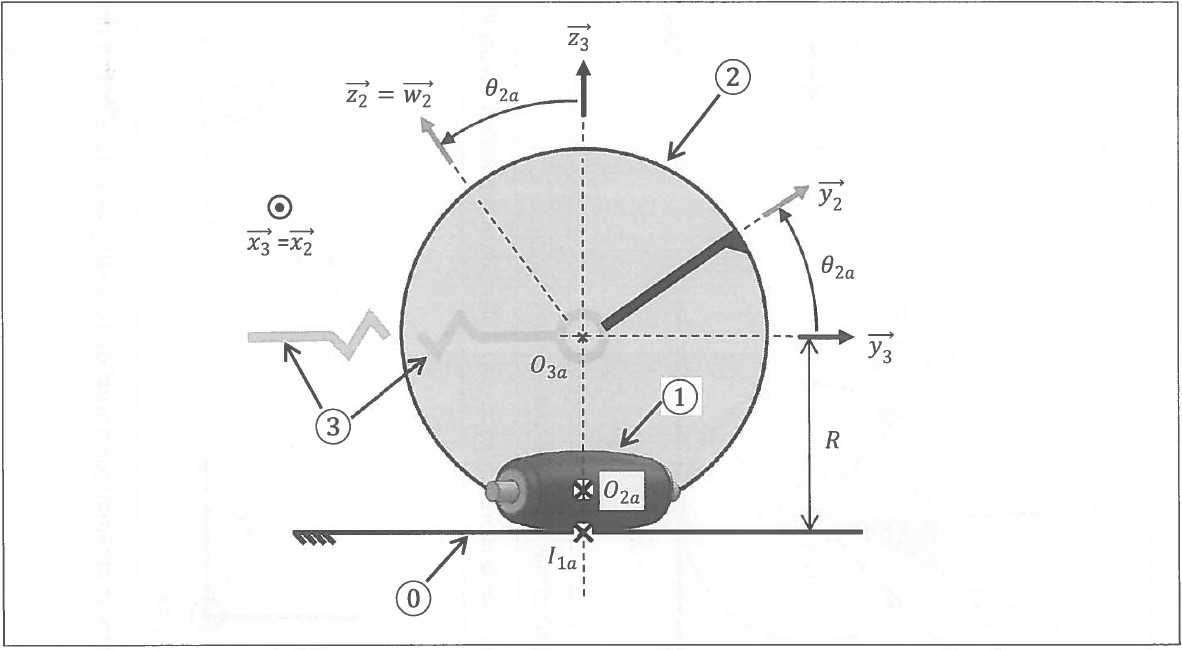
\includegraphics[width=\textwidth]{fig_05}
\caption{Evolution de $S_D$ sur un pas de marche\label{ccs_psi_2023_fig_05}}
\end{figure}

\fi


%Q4
\question{\label{ccs_psi_2023_q_04} 
 À partir de la figure \ref{ccs_psi_2023_fig_05}, déterminer, parmi les valeurs proposées, l'erreur maximale admissible sur les axes $S_{\theta, \max }$ de l'exosquelette Atalante afin d'éviter la chute du patient.}
\ifprof
\begin{corrige}
D'après le cahier des charges, l'incertitude de la position du point
$D$ par rapport au point  $A$  doit être au maximum de $\SI{5}{mm}$. Parmi les 4 figures, seule une incertitude $S_{\theta}=\SI{0,01}{rad}$ permet d'avoir une incertitude $S_D < \SI{5}{mm}$.
\end{corrige}
\else
\fi

\ifprof
\else
Quel que soit le résultat trouvé à la question précédente, une erreur maximale admissible de \SI{0,01}{rad} pour chacun des axes sera considérée pour la suite.

Afin de respecter l'exigence sur l'erreur maximale admissible, des asservissements de position et de vitesse ont été élaborés pour chacun des axes sans prendre en compte l'éventuelle influence du couplage entre les axes.

Des essais ont alors été effectués afin de mesurer l'évolution réelle des angles de chaque axe par rapport à la trajectoire visée. La figure 6 montre l'évolution de l'erreur pour l'axe de hanche sagittal de la jambe gauche lors d'une marche en ligne droite.
\fi

%Q 5
\question{\label{ccs_psi_2023_q_05}  À partir de la figure \ref{ccs_psi_2023_fig_06} et en justifiant la réponse, conclure sur la capacité des asservissements réalisés sans prise en compte du couplage entre les axes à respecter l'exigence 1.2.1.1.}
\ifprof
\begin{corrige}
L'exigence indique que <<~Le talon doit être positionné à moins de
\S{5}{mm} de la consigne~>>. Pour cela on a vu que l'erreur maximale admissible sur chacun des axes doit être inférieure à \SI{0,01}{rad}. À tout stade de la marche, cette erreur est ici supérieure à \SI{0,01}{rad}. Les asservissements élaborés ne conviennent donc pas.
\end{corrige}
\else
\fi

\ifprof
\else

\begin{figure}[!h]
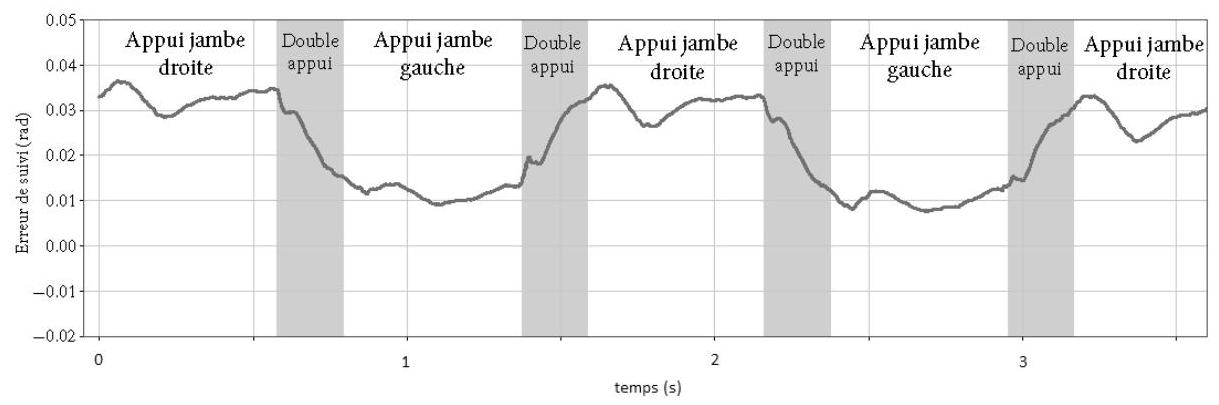
\includegraphics[width=\textwidth]{2023_05_12_54c6a64d2ffce28d5c72g-04(3)}
\caption{Évolution de l'erreur pour l'axe de hanche sagittal de la jambe gauche\label{ccs_psi_2023_fig_06}}
\end{figure}
\fi



